\documentclass[nobib]{tufte-handout}
%\usepackage{etex} \reserveinserts{36}
\usepackage{graphicx}
\usepackage{morefloats}
\usepackage{cite}
\setkeys{Gin}{width=\linewidth,totalheight=\textheight,keepaspectratio}
\graphicspath{{figures/}}
\usepackage{booktabs}

% \definecolor{dark2orange}{HTML}{D95F02}  % Dark2 Orange
% \definecolor{dark2green}{HTML}{1B9E77}   % Dark2 Green
% \definecolor{dark2purple}{HTML}{7570B3}  % Dark2 Purple

\definecolor{dark2orange}{HTML}{E6550D}  % More saturated orange
\definecolor{dark2green}{HTML}{138D75}   % Darker green
\definecolor{dark2purple}{HTML}{6A51A3}  % Richer purple

\definecolor{darkblue}{HTML}{002147}
\hypersetup{citecolor=darkblue, linkcolor=black, urlcolor=blue}

% The fancyvrb package lets us customize the formatting of verbatim
% environments.  We use a slightly smaller font.
\usepackage{fancyvrb}
\fvset{fontsize=\normalsize}

% Small sections of multiple columns
% \usepackage{multicol}

\hypersetup{colorlinks}

\newcommand{\minisec}[1]{\vspace{3pt} \noindent \emph{#1}\ }

\title{Inviting Darwin into protein foundation models}
\author{\href{http://matsen.fredhutch.org/}{Frederick A. Matsen}, Fred Hutchinson Cancer Center}


\begin{document}

\maketitle

\begin{abstract}
\noindent
Language models of protein sequences have tremendous promise for understanding and predicting the function of protein variants.
However, the current generation of models ignore evolutionary biology.
We have shown that by placing deep neural networks inside a classical mutation-selection framework for antibodies, we obtain a model that does much better at functional prediction, as well as being more interpretable, 10x smaller, and 500x faster.
Moving forward, we will extend this approach to other systems, most ambitiously to all proteins.
\end{abstract}

\newthought{Evolution is a process of mutation and selection.}
Current protein language models ignore this fact.
Indeed, such models are trained using a masked loss on observed protein sequences, which removes the protein from the phylogenetic context in which it arose, and ignores the nucleotide-level processes that lead to evolution.

\begin{marginfigure}[-9.9cm]%
  \hspace{-19pt}
  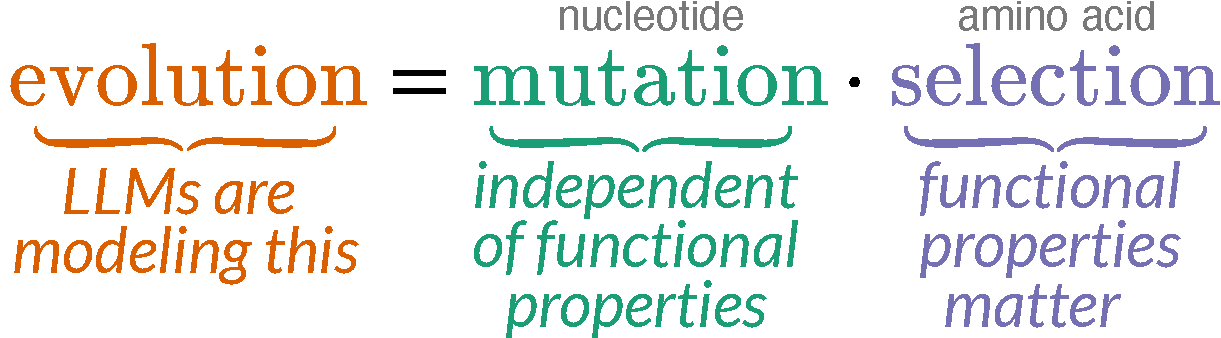
\includegraphics[width=2.4in]{figures/evolution-is-mut-and-sel.why.pdf}%
  \caption{the Darwinian perspective}
  \label{fig:darwin}
\end{marginfigure}

Our specialty is the evolution of antibodies, and we have seen these effects in antibody language models.
Although antibody language models are benchmarked for functional prediction~\cite{Chungyoun2024-fc}, nucleotide-level effects are obvious when one looks for them.
For example, AbLang2~\cite{Olsen2024-ablang2} estimates amino acids coded for by codon neighbors as being two orders more likely than non-neighbors.
The effect of neutral mutation probability is also evident (Figs~\ref{fig:codon} \& \ref{fig:neutral}).

\begin{marginfigure}[-7.8cm]%
  \hspace{-19pt}
  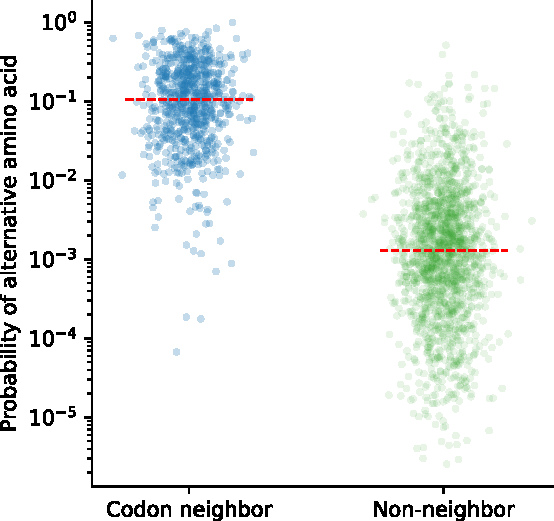
\includegraphics[width=2.0in]{figures/ablang2-neighbor-csp.pdf}%
  \caption{AbLang2 probabilities}
  \label{fig:codon}
\end{marginfigure}

These factors negatively impact functional prediction for these models.
For example, AbLang2's correlation with expression data~\cite{Koenig2017-vm} drops from 0.49 for codon neighbors to 0.30 for non-neighbors, and when put together the correlation is only 0.34.
The results for benchmark binding assays are significantly worse.

\begin{marginfigure}[-1.2cm]%
  \hspace{-19pt}
  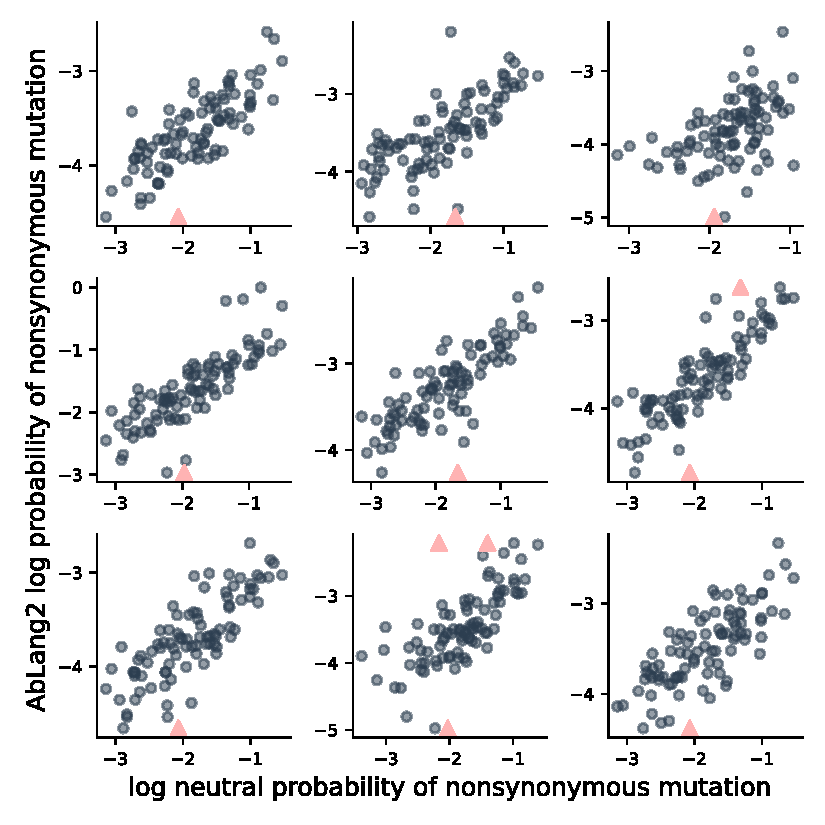
\includegraphics[width=2.4in]{figures/ablang2-vs-neutral.pdf}%
  \caption{neutral probs vs LLM probs}
  \label{fig:neutral}
\end{marginfigure}

\subsection*{A deep natural selection model is a win on all fronts}

Rather than fitting a combined model of mutation and selection, we can fit separate models in a manner exactly mirroring Figure~\ref{fig:darwin}:
\begin{equation}
\color{dark2orange}{m_{j,c}(t, P)} = \color{dark2green}{p_{j,c}(t, P)} \cdot \color{dark2purple}{f_{j,\bar{c}}(\bar{P})}.
\label{eq:darwin}
\end{equation}
Here $c$ is a codon, $j$ is a site, $t$ is time, and P is a parent sequence. 
%Bar denotes amino acid translation.

\begin{marginfigure}[0.2cm]%
  \hspace{-19pt}
  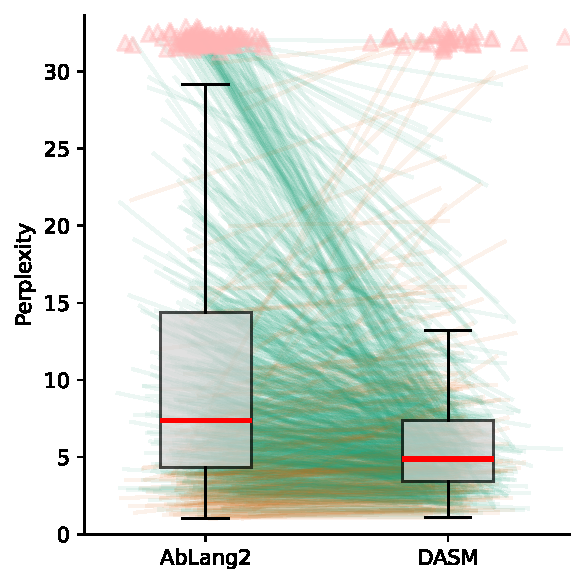
\includegraphics[width=2in]{figures/perplexity_comparison-v1rodriguez}
  \caption{model fit (lower = better)}
  \label{fig:perplexity}
\end{marginfigure}


This is a higher-resolution and modern version of foundational models from 25 years ago~\cite{Halpern1998-yc}.
The mutation term $\color{dark2green}{p_{j,c}(t, P)}$ is a convolutional neural network modeling the neutral mutation process~\cite{thrifty} and the selection term $\color{dark2purple}{f_{j,\bar{c}}(\bar{P})}$ is a transformer-encoder neural network of modest size.
Rather than training using an abiological masked-modeling objective, our objective is to predict the location and identity of mutations in the evolution of antibodies.

This Deep Amino acid Selection Model (DASM) performs better according to every metric.
It has better model fit (Figure~\ref{fig:perplexity}).
It also performs better on functional benchmark tasks (Table~\ref{tab:model-comparison}).
It is an order of magnitude smaller than the smallest modern antibody language model, trained on orders of magnitude less data, and 500x faster to run.
The models are readily interpretable (Figure~\ref{fig:interpretation}).
\begin{table}[ht]
    \begin{tabular}{lccccc}
    & AbLang2 & ESM & ProGen2 & DASM \\
    \midrule
    Koenig G6 Binding~\cite{Koenig2017-vm} & -0.032 & -0.001 & 0.156 & \textbf{0.312} \\
    Koenig G6 Expression~\cite{Koenig2017-vm} & 0.344 & 0.418 & 0.559 & \textbf{0.669} \\
    Shane. binding 119~\cite{Shanehsazzadeh2023-qe} & 0.263 & 0.248 & 0.074 & \textbf{0.470} \\
    Shane. binding 120~\cite{Shanehsazzadeh2023-qe} & 0.166 & 0.337 & 0.052 & \textbf{0.540} \\
    \bottomrule
    \end{tabular}
    \caption{Correlation of models with functional measurements on the biggest benchmark datasets from~\cite{Chungyoun2024-fc}.
    Competitor models include AbLang2~\cite{Olsen2024-ablang2} as well as leading protein LLMs ESM~\cite{Rives2021-la} and ProGen2~\cite{Nijkamp2022-fy}.
    ProGen2 has been shown overall to be best existing model at functional prediction tasks~\cite{Chungyoun2024-fc}.
    }
    \label{tab:model-comparison}
  \end{table}

\section{Future work}

\paragraph{Short term}
Thus far, we have been entirely focused on model formulation and now will move into a phase of scale-up and model refinement. We will scale to bigger models on larger data sets. We will also work on antigen-specific models, using clonal family structure and antigen-specific data.

\begin{marginfigure}[1.3cm]%
  \hspace{-7pt}
  \includegraphics[width=2in]{figures/conserved-D-end-of-CDR3.png}
  \caption{Our model predicts the importance of an aspartic acid near the end of the antibody heavy CDR3, which can be seen making structurally-important stabilizing interactions.}
  \label{fig:interpretation}
\end{marginfigure}

\paragraph{Medium term}
We will fit models in other settings with many closely related sequences, such as for influenza and SARS-CoV-2.
We already have a neutral model for SARS-CoV-2~\cite{Haddox2025-ej}.
The resulting fitness predictions will be much higher resolution than existing models (e.g.~\cite{Bloom2023-af}) and naturally incorporate deep mutational scans.

\paragraph{Long term}
We will develop general-purpose protein selection models.
There is nothing in our formulation (\ref{eq:darwin}) that is specific to viruses or the immune system.
This will require us to do phylogeny and ancestral sequence reconstruction on massive scale.
We will be competing with startups such as \href{https://www.evolutionaryscale.ai/}{EvolutionaryScale}, which recently got \$142M in VC funding, and builds closed-source models.

\section{Impact}
Our open-source models will accurately capture the \emph{functional} aspects of protein evolution across domains. 
As for antibodies, they will be more accurate, smaller, faster, and more interpretable.

More generally, we want to help bring biology back into the center of biological foundation models.
% The entire scientific community benefit from better-performing and biologically-relevant open-source models.




\newpage
\bibliography{main}
\bibliographystyle{tufte}

\end{document}


% ,matsen2012ubiquity
